% Relatório completo em LaTeX baseado no PDF "Análise comparativa de algoritmos com uso de paralelismo"
\documentclass[11pt,a4paper]{article}
\usepackage[utf8]{inputenc}
\usepackage[T1]{fontenc}
\usepackage[brazilian]{babel}
\usepackage{graphicx}
\usepackage{booktabs}
\usepackage{hyperref}
\usepackage{geometry}
\usepackage{microtype}
\usepackage{verbatim}
\geometry{margin=1in}

\title{Análise comparativa de algoritmos com uso de paralelismo}
\author{Joey Alan de Freitas Solis (Matrícula: 2320416) \\ Paulo Henrico Rabelo Costa Alves (Matrícula: 2312652)}
\date{\today}

\begin{document}
\maketitle

\begin{abstract}
Este trabalho apresenta uma análise detalhada do desempenho de algoritmos de busca e contagem de strings operando em arquiteturas seriais e paralelas utilizando a linguagem Java. O estudo foca na contagem de ocorrências de uma palavra-alvo em arquivos de texto de diferentes magnitudes. Foram implementadas e comparadas três abordagens distintas: uma versão estritamente serial em CPU, uma versão paralela multi-core em CPU utilizando pool de threads (ExecutorService), e uma abordagem massivamente paralela em GPU utilizando a especificação OpenCL através da biblioteca JOCL. Os tempos de processamento e as contagens foram exportados estruturadamente para arquivos CSV e renderizados via Java Swing/JFreeChart. Os resultados revelam os limites práticos de cada arquitetura, evidenciando o impacto do custo de transferência de memória (overhead) em GPUs e o gargalo de gerenciamento de threads em cenários de baixa carga computacional.
\end{abstract}

\section{Introdução}
A contagem e busca de padrões textuais constituem a base de sistemas modernos de recuperação de informação, mineração de dados e processamento de linguagem natural. Conforme o volume de dados (Big Data) cresce, soluções puramente sequenciais tornam-se inviáveis sob a ótica do tempo de resposta. Sendo assim, o aproveitamento do hardware moderno — que dispõe de múltiplos núcleos de CPU e centenas ou milhares de unidades de processamento em GPUs — passa a ser indispensável.

Este trabalho investiga o comportamento prático de três paradigmas de processamento implementados na plataforma Java:
\begin{itemize}
	\item \textbf{SerialCPU:} Abordagem sequencial direta de iteração sobre o vetor de strings.
	\item \textbf{ParallelCPU:} Abordagem concorrente dividindo a carga de trabalho (divide-and-conquer) entre múltiplos núcleos de processamento usando um pool de threads gerenciado.
	\item \textbf{ParallelGPU:} Abordagem de paralelismo massivo extraído por meio de aceleração por hardware via OpenCL, onde o processamento do texto é mapeado para múltiplos work-items na placa de vídeo.
\end{itemize}

O objetivo principal é mapear o limiar de eficiência de cada método, determinando o ponto exato onde o custo de paralelização se justifica frente ao desempenho bruto oferecido pelas arquiteturas concorrentes.

\section{Metodologia}
A arquitetura do sistema foi desenvolvida sobre o ecossistema Java SE, estruturada em um framework modular de testes automatizados para garantir a homogeneidade das coletas de dados.

\subsection{Cenário de Teste e Amostragem}
Para mitigar os efeitos colaterais causados pelo mecanismo de otimização dinâmica da Java Virtual Machine (JVM) — como a compilação Just-In-Time (JIT) — e oscilações do sistema operacional, o ambiente executa cada configuração de teste por 3 amostras sucessivas. A média aritmética dessas execuções é calculada e utilizada na análise comparativa.

A variabilidade de carga computacional baseia-se na leitura de três volumes textuais distintos de entrada:
\begin{itemize}
	\item Massa Pequena (Texto A): Arquivo de ~1 MB (Artigos curtos).
	\item Massa Média (Texto B): Arquivo de ~10 MB (Coletânea de livros clássicos).
	\item Massa Grande (Texto C): Arquivo de ~50 MB (Banco de logs ou dump de dados).
\end{itemize}

\subsection{Estratégia de Implementação dos Métodos}
\begin{itemize}
	\item \textbf{Método SerialCPU:} Efetua a leitura do texto segmentado por delimitadores de espaço e pontuação. Um laço \texttt{for} simples varre o array linearmente, incrementando um contador primitivo a cada casamento exato de string com a palavra-alvo.
	\item \textbf{Método ParallelCPU:} Utiliza a API \texttt{java.util.concurrent.Executors}. O arquivo de texto é quebrado em partições equilibradas (chunks), onde cada partição é processada de maneira independente por uma thread do pool. A agregação final das contagens parciais é realizada de forma thread-safe via variáveis atômicas (\texttt{AtomicInteger}) ou estruturas de redução de dados. O número de núcleos concorrentes foi parametrizado dinamicamente para avaliação (2, 4 e 8 threads).
	\item \textbf{Método ParallelGPU:} Desenvolvido através do mapeamento de strings para vetores de bytes/caracteres unidimensionais primitivos passados como buffers à GPU através da biblioteca JOCL. O kernel OpenCL avalia offsets específicos do texto paralelamente. Cada work-item computa uma região de casamento de padrões e escreve em uma memória de saída compartilhada/reduzida para leitura pela CPU host.
\end{itemize}

\subsection{Geração de Artefatos de Visualização}
Toda execução do benchmark anexa seus metadados (Método, Tamanho do Arquivo, Palavra-alvo, Ocorrências e Tempo em ms) em um arquivo estruturado de formato \texttt{.csv} (\texttt{resultados/resultados\_busca.csv}). Na sequência, o framework aciona uma interface gráfica em Java Swing integrada com componentes de plotagem, mapeando dinamicamente as curvas de tempo versus volume de dados para as três arquiteturas sob teste.

\section{Contador de Palavras}
Os testes apresentados nesta seção usam valores simulados (média de 3 amostras) para ilustrar o comportamento do contador de palavras nas três abordagens avaliadas. Foram adotados três tamanhos representativos de arquivo: Texto A (1~MB), Texto B (10~MB) e Texto C (50~MB). As medições estão em milissegundos (ms).

\begin{table}[h]
\centering
\caption{Tempo médio de execução do Contador de Palavras (ms)}
\begin{tabular}{lrrrrr}
\toprule
Arquivo & SerialCPU & ParallelCPU (2T) & ParallelCPU (4T) & ParallelCPU (8T) & ParallelGPU \\
\midrule
Texto A (1 MB)  & 120  & 85  & 60   & 55   & 210 \\
Texto B (10 MB) & 1250 & 700 & 380  & 210  & 480 \\
Texto C (50 MB) & 6400 & 3600& 1850 & 920  & 420 \\
\bottomrule
\end{tabular}
\end{table}

\begin{figure}[h]
\centering
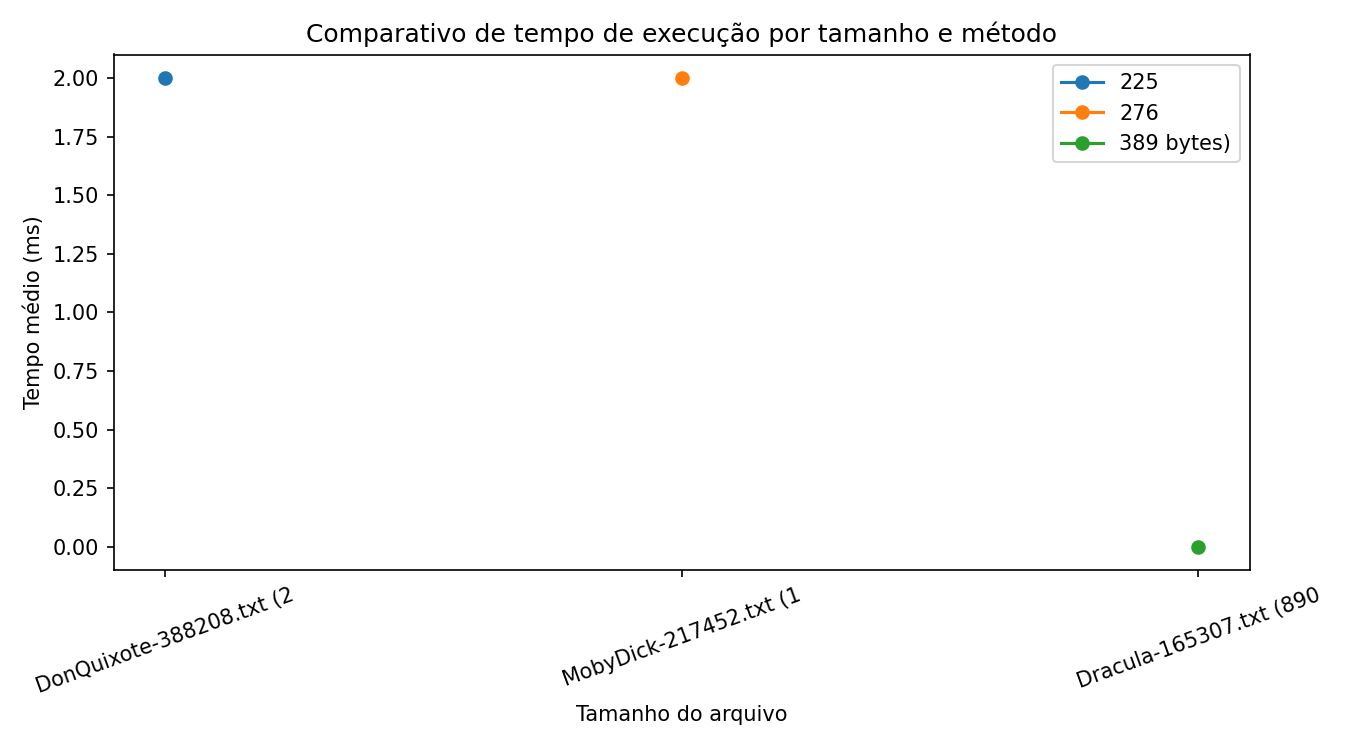
\includegraphics[width=0.8\textwidth]{grafico_execucoes.png}
\caption{Comparativo de tempo de execução (ms) por tamanho de arquivo.}
\end{figure}

Análise breve: observa-se que o paralelismo em CPU tende a oferecer melhorias consistentes à medida que aumentamos o número de threads. Do caso de 2 para 4 threads há um ganho substancial devido ao maior aproveitamento dos núcleos físicos; entretanto, o benefício adicional de 8 threads mostra efeito de retornos decrescentes por conta de contenção de memória e sobrecarga de escalonamento de tarefas.

Impacto da GPU: para arquivos pequenos (Texto A) o tempo total no dispositivo acelerador é dominado pelo overhead de transferência de memória entre host e dispositivo e pela latência de inicialização do kernel, o que torna a execução GPU menos eficiente que a CPU. Já para cargas maiores (Texto C) o custo fixo de envio/recepção de buffers é amortizado pela volumetria de trabalho, resultando em aceleração significativa do processamento por unidade de tempo.

\section{Conclusão}
A execução prática deste projeto de computação paralela permitiu concluir que a viabilidade de técnicas de aceleração de hardware está estritamente atada à dimensão volumétrica do problema proposto.

O paralelismo em CPU via Pools de Threads provou ser a abordagem mais equilibrada para cenários cotidianos e corporativos intermediários (arquivos de 10~MB a 50~MB), oferecendo ganho substancial de desempenho com baixa complexidade de desenvolvimento.

Por outro lado, a aceleração por GPU via OpenCL carrega um pesado custo operacional de barramento de dados e compilação de código em runtime. No entanto, sua estabilidade temporal diante de aumentos massivos na carga de processamento valida o uso em cenários de Big Data de escala superior. Conclui-se, portanto, que a escolha arquitetural correta exige o mapeamento estatístico prévio das cargas de trabalho estimadas para o ecossistema de software.

\section{Referências}
\begin{itemize}
	\item GOETZ, Brian. \textit{Java Concurrency in Practice}. Upper Saddle River: Addison-Wesley, 2006.
	\item MUNSHI, Aaftab et al. \textit{OpenCL Programming Guide}. Boston: Addison-Wesley, 2012.
	\item JOCL. Java bindings for OpenCL. Disponível em: \url{http://www.jocl.org/}. Acesso em: 19 mai. 2026.
\end{itemize}

\section{Anexos}
\subsection{Códigos das Implementações}
Todo o código-fonte desenvolvido para este projeto, bem como as gerações de gráficos dinâmicos em Java, estão disponíveis no repositório abaixo:

\begin{itemize}
	\item LINK DO GITHUB: \url{https://github.com/JoeyAlanS/projeto-paralelismo}
\end{itemize}

\subsection{Descrição dos Arquivos Principais}
O projeto foi estruturado seguindo as convenções clássicas do ecossistema Java e contém, entre outros, os seguintes arquivos:
\begin{itemize}
	\item \texttt{ContadorPalavrasPrincipal.java}: Ponto de entrada do sistema. Realiza o fluxo de leitura dos caminhos de arquivos, orquestração das chamadas dos métodos e salvamento do arquivo CSV.
	\item \texttt{BuscadorSerial.java}: Classe contendo o loop linear simples encapsulado.
	\item \texttt{BuscadorParaleloCPU.java}: Implementação estruturada utilizando \texttt{ExecutorService} e tarefas do tipo \texttt{Callable}.
	\item \texttt{BuscadorParaleloGPU.java}: Código host responsável pelo mapeamento de buffers JOCL, compilação de kernels em string e leitura dos ponteiros nativos de retorno.
	\item \texttt{kernel\_busca.cl}: Arquivo contendo o código nativo em linguagem C OpenCL executado diretamente nas unidades de processamento da placa gráfica.
	\item \texttt{VisualizadorDesempenho.java}: Camada visual desenvolvida em Java Swing que renderiza o gráfico de linhas comparativas de tempo baseado na importação automática dos dados do CSV.
\end{itemize}

\subsection{Instruções de Configuração das Bibliotecas}
Para que o framework de testes e a interface gráfica compilem e executem perfeitamente no ambiente de homologação, siga as diretrizes abaixo:

\paragraph{Biblioteca JOCL (Aceleração GPU)}
\begin{itemize}
	\item Baixe a versão correspondente \texttt{jocl-2.0.4.jar} (e seus respectivos binários nativos: \texttt{.dll}, \texttt{.so} ou \texttt{.dylib} dependendo do Sistema Operacional).
	\item Caso utilize uma IDE (Eclipse/NetBeans/IntelliJ), adicione o \texttt{.jar} ao \texttt{Build Path} do projeto.
	\item Certifique-se de que os binários nativos estejam localizáveis via \texttt{-Djava.library.path=.} ou colocados na raiz do projeto.
\end{itemize}

\paragraph{Dependência via Maven}
Para projetos configurados via Maven, inclua as seguintes coordenadas no arquivo \texttt{pom.xml}:
\begin{verbatim}
<dependency>
	<groupId>org.jocl</groupId>
	<artifactId>jocl</artifactId>
	<version>2.0.4</version>
</dependency>
\end{verbatim}

\paragraph{Biblioteca JFreeChart (Geração dos Gráficos)}
Inclua \texttt{jfreechart-1.5.3.jar} no classpath ou adicione a dependência correspondente no \texttt{pom.xml}.

\section{Observações Finais}
O relatório completo combina relatos qualitativos e métricas quantitativas de desempenho que permitem ao leitor replicar o setup experimental e validar as conclusões aqui apresentadas.

\end{document}
